\documentclass[12pt]{report}
\usepackage[utf8]{inputenc}
\usepackage{cite}
\usepackage[hidelinks]{hyperref}
\usepackage{graphicx}
\usepackage{amsfonts}
\usepackage{mathtools}
\usepackage{caption}
\usepackage{fancyhdr}

\pagestyle{fancy}
\fancyhf{}
\rhead{ODE Solver Design}
\lhead{\thesection}
\rfoot{\thepage}

\DeclarePairedDelimiter\ceil{\lceil}{\rceil}
\DeclarePairedDelimiter\floor{\lfloor}{\rfloor}

\title{\textbf{ODE Solver Design Report}}
\author{
  Mahmoud Adas\\
  \small\texttt{SEC:2, BN:21}
  \and
  Evram Youssef\\
  \small\texttt{SEC:1, BN:9}
  \and
  Remonda Talaat\\
  \small\texttt{SEC:1, BN:20}
  \and
  Mohamed Shawky\\
  \small\texttt{SEC:2, BN:16}
}
\date{\today}

\begin{document}

\thispagestyle{empty}

\maketitle
\tableofcontents
\listoffigures
\listoftables
\clearpage

\pagenumbering{arabic}

\part{Introduction}
\section{Abstract}
This is phase 1 design report for VLSI project. 

This document is intended to be used as a comprehensive reference for the coming phases, and to be up-to-date with all future changes in the design.

\section{Team and Tasks}
Table \ref{tab:tasks} contains all tasks, the team-member who took that task and the time it took them to finish.
\begin{table}
    \captionof{table}{Tasks Distribution\label{tab:tasks}}
 \begin{tabular}{||p{30mm}| p{40mm}| p{15mm}| p{40mm}||} 
 \hline
 Task & Members & Duration \newline (hours) & Challenges  \\ [0.5ex] 
 \hline\hline
 Overall system design & Mahmoud Othman \newline Evram Youssef \newline Remonda Talaat \newline Mohamed Shawky & 20-25 & - Understanding the problem definition. \newline - Making a lot of assumptions. \\
 \hline
 External Interface of Each component & Mohamed Shawky & 3-4 & Redesigning interface with internal changes. \\ 
 \hline
 Assumption and limitation & Remonda Talaat  & 2-3 & Recalculation with every change made. \\
 \hline
 Overall system scenario & Mahmoud Othman & 2-3 & The tool to use to illustrate the design with. \\
 \hline
 Memory sizes & Evram Youssef & 1-2 & Making large/huge assumptions where it's not required. \\
 \hline
 Parallelism and Pipeline & Evram Youssef & 1-2 & Not knowing for sure if a proposal will work or not. \\
 \hline
 Communication between modules & Mahmoud Othman & 2-3 & Deciding the necessary sizes. \\
 \hline
 Address mapping & Remonda Talaat & 2-3 & Redesigning. \\
 \hline
 Sub-components and Buses & Evram Youssef & 2-3 & Understanding in details the job of each module. \\
 \hline
 Creating the documentation & Mahmoud Othman \newline Evram Youssef \newline Remonda Talaat \newline Mohamed Shawky & 8-10 & - Redundancy. \newline - Unifying style. \\
 \hline
 Styling the documentation & Mahmoud Othman \newline Mohamed Shawky & 4-5 & --------------------------- \\
 \hline\hline
\end{tabular}
\end{table}

\section{Interfaces and Actions}
\begin{center}
    \begin{figure}[hp]
        \centering
        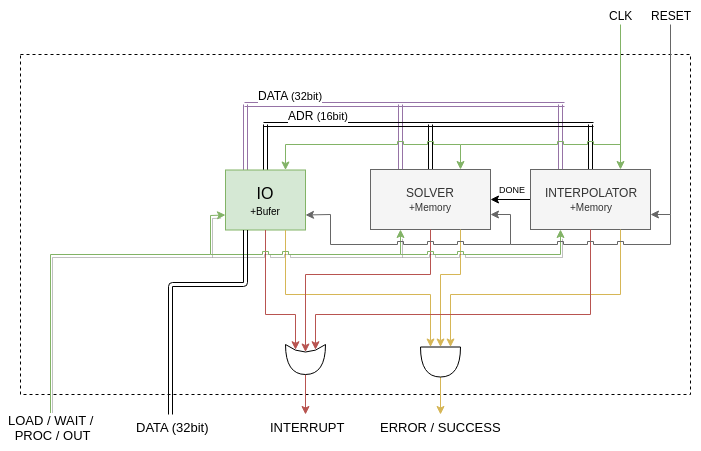
\includegraphics[width=\textwidth]{d1}
        \caption{Overall System Design}
        \label{fig:overall}
    \end{figure}
\end{center}

The main module, as shown in Figure \ref{fig:overall}, has the ports listed in Subsection \ref{sec:interface:ports} that triggers some actions. 

Ports and their actions are summarized below and detailed in the rest of the document.

\subsection{Ports}
\label{sec:interface:ports}

\subsubsection{CLK: IN}

\subsubsection{RESET: ASYNC IN}
\begin{itemize}
    \item clears all internal states of all modules:
    \begin{itemize}
        \item IO internal buffer.
        \item ERROR/SUCCESS of all modules resets to SUCCESS.
        \item INTERRUPT resets to zero.
    \end{itemize}
    \item Memory at solver and interpolator are NOT cleared.
    \item At next clock, CPU is expected to turn the {LOAD / WAIT / PROC / OUT} into {LOAD} state and we will start loading input again.
\end{itemize}

\subsubsection{LOAD / WAIT / PROC / OUT (2bit): IN}
Set the current major state of the machine.
\begin{itemize}
    \item LOAD(0):
    \begin{itemize}
        \item IO receives \textbf{compressed} data from the CPU.
        \item IO decompresses data into buffer.
        \item buffer is flushed into data bus with appropriate address.
        \item ends when cpu finishes its data loading and switches to {WAIT} state.
    \end{itemize}
    \item WAIT(1):
    \begin{itemize}
        \item Same state as {LOAD}, but IO doesn't receive anymore data from CPU.
        \item ends when IO flushes all its buffer and raises {INTERRUP} with either {ERROR} or {SUCCESS}.
    \end{itemize}
    \item PROC(2):
    \begin{itemize}
        \item SOLVER sends time step to calculate {U} at.
        \item SOLVER and INTERPOLATOR work concurrently to calculate their outputs.
        \item INTERPOLATOR sends {DONE} signal to SOLVER when it finishes the interpolated U.
        \item SOLVER can request to copy the interpolated {U}.
        \item INTERPOLATOR waits for SOLVER to send next time step.
        \item ends when either SOLVER or INTERP raises INTERRUPT with either {SUCCESS} or {ERROR}.
    \end{itemize}
    \item OUT(3):
    \begin{itemize}
        \item IO just copies final outputs to cpu from SOLVER memory.
        \item ends when IO raises INTERRUPT with either {SUCCESS} or {ERROR}.
    \end{itemize}
\end{itemize}

\subsubsection{DATA (32bit): INOUT}
\begin{itemize}
    \item Data bus between cpu and io.
\end{itemize}

\subsubsection{INTERRUPT: OUT}
\begin{itemize}
    \item Raised from 0 to 1 when some internal module (IO / SOLVER / INTERPOLATOR) finishes its task.
    \item If task finished with success the {ERROR / SUCCESS} is set to {SUCCESS}, otherwise it's {ERROR}.
\end{itemize}

\subsubsection{ERROR(0) / SUCCESS(1): OUT}
\begin{itemize}
    \item CPU should operate on this value ONLY when {INTERRUPT} is 1.
    \item Errors that could happen include: divide by zero, H > 1, incomplete input.
\end{itemize}

\section{Parallelism in Design} 
\label{sec:parallel}  
Parallelism takes place when the solver is calculating the next $X_h$ and interpolator is calculating $U_h2$.

\subsection{Possible Problems}
\subsubsection{In Fixed Step Mode} 
The only problem is when the unit reachs the last $X$, then the upcoming $h$ will be garbage or unwanted $h$, and the unit will terminate either ways.

\subsubsection{In Adaptive/Variable Step Mode} 
When solver is calculating $X_h$, interpolator is busy calculating $U_{h/2}$, and when solver is calculating $X_{h/2}$ and $X_{h}$, interpolator will be calculating $U_{h}*$, $h*$ is the $h$ from the algorithm equation, which is $h = \frac{0.9 \times h^2 \times L}{e}$, this $U_{h}$* might not even be used, and then, solver will interrupt the interpolator, and orders it to calculate $U_{hnew}$.

\section{Inter-module Communication}

\subsection{IO and CPU}
\begin{itemize}
    \item CPU orders to Load, IO reads 32bits of data.
    \item When CPU finishes, raises WAIT, when IO finishes that last package of data int the cpu with success.
    \item CPU raises PROC, so that all of other components starts acting.
    \item When output data is ready, CPU is interrupted with error or success, then CPU raises OUT signal which implies that it's ready to take out the resulting output from IO.
    \item If there's an error, CPU should know which component sent it.
\end{itemize}

\subsection{IO and Solver/Interpolator}
\begin{itemize}
    \item IO puts the data and address on their busses, each component of them two reads that address and check if this address is within its range, if so this component reads the data and stores it.
    \item When Solver is ready to flush the result it raises int and success or even error.
\end{itemize}

\subsection{Solver and Interpolator}
\begin{itemize}
    \item See Section \ref{sec:parallel}.
    \item Solver is working on $X_h$ so it needs U, solver checks on DONE signal, if raised, reads the U from the data bus, Interpolator has already placed it there.
    \item Then Solver places h$_new$ at the data bus, interpolator reads it and they both work...
    \item and repeat.
\end{itemize}

\part{Simulation Workflow}
\section{Input Preprocessing}
This stage is the responsibility of a script that runs before the simulation:
\subsubsection{Stage Input}
JSON file that follows the format stated in the main project document \cite{mainDoc}.

\subsubsection{Steps}
\begin{itemize}
    \item Create bit stream of the read data that follows the {Input Data Structure} specifications.
    \item encode the bits following the {Compression} specifications.
    \item Collect encoding output in ASCII string, each byte in string is either '0' or '1' in ASCII format.
    \item When the string reaches the length of 32 bytes, push it to output file.
    \item If the last created string didn't reach the length of 32 bytes, complete the rest with '0' and push it to the output file.    
\end{itemize}

\subsubsection{Stage Output}
\begin{itemize}
    \item ASCII file that contains multiple lines of compressed data.
    \item each line has exactly 32 '0' or '1' ASCII characters.
    \item ONLY the ASCII characters 0 or 1 are permitted in the file and NOTHING ELSE.
    \item there is NO EMPTY LINE/s in the file or spaces.
\end{itemize}

\section{Instantiating Main Module}
This stage and all the next ones are the responsibility of the CPU simulation code.

CPU is a non-synthesisable HDL test-bench that:
\begin{itemize}
    \item Instantiates the HW main module.
    \item Attaches the appropriate signals to the HW main module.
    \item Generates CLK with fixed frequency.
    \item Loads data into HW.
    \item Puts HW into PROCESS state.
    \item Load output out from the HW and into a file.
\end{itemize}

\section{Input Loading}
\begin{itemize}
    \item Load the output of the former script into array of vectors each is 32bit wide that will hold one line in the file.
    \item Put HW at LOAD state.
    \item RESET for one cycle.
    \item For each 32bit vector in the former array:
    \begin{itemize}
        \item At the positive edge of CLK:
        \begin{itemize}
            \item Load vector into DATA bus.
        \end{itemize}
    \end{itemize}
    \item Load DATA with 0s.
    \item Wait for the positive edge of INTERRUPT signal.
    \item Check for ERROR / SUCCESS and only proceed if it is SUCCESS.
\end{itemize}

\section{Processing}
\begin{itemize}
    \item Put HW at PROCESS state.
    \item Wait for the {INTERRUPT} positive edge.
    \item Check for {ERROR / SUCCESS} and only proceed if it is SUCCESS.
\end{itemize}

\section{Output Extraction}
\begin{itemize}
    \item Put high impedance on {DATA} bus.
    \item Put HW at OUT state.
    \item Keep receiving data into array of vectors and outputting them into file in the same format of the input file.
    \item Wait for the positive edge of {INTERRUPT} signal. 
\end{itemize}

Simulation is done! 

You can turn the output into human-readable json using output-formatting script.

\part{Specifications}

\section{Memory Mapping}
The Following addresses are only meant for internal communicating between modules, and they don't need to resemble actual addresses stored at some memory. 

The address loaded at the bus resembles what kind of data is on data bus or what kind of data this module should output.

If address bus is loaded with an address \emph{Adr} that some module \emph{M} is not assigned to, module \emph{M} must ignore the data and address bus so the rest can communicate.

This way communication is simplified.

\emph{A} column for module \emph{M} is the action of the address taken at module \emph{M} when it sees that address. It's either:

\begin{itemize}
    \item \emph{W}: \textbf{Write to} module \emph{M}. Module \emph{M} is expected to \textbf{read} the data bus and store data internally, so the other module \emph{wrote} to module \emph{M}.
    \item \emph{R}: \textbf{Read from} module \emph{M}. Module \emph{M} is expected to \textbf{write} some data to the data bus as response to this address, so the other module \textbf{reads} from it.
\end{itemize}

\subsection{Solver Memory Mapping}
Solver module listens at the addresses listed in Table \ref{tab:solver-mem}.

\begin{center}
    \captionof{table}{Solver Memory Mapping\label{tab:solver-mem}}
 \begin{tabular}{||c| c| c| c| c| l||} 
 \hline
 Address & A & Type & Words & Name & Description  \\ [0.5ex] 
 \hline\hline
  0x0000 & W & \emph{struct Header} & 1 & Header & Includes Dimensions and modes  \\ 
 \hline
 0x0001  & W & f64 & 4 & H & Timestep (variable step mode)  \\
 \hline
 0x0005  & W & f64 & 4 & Error & Error Tolerance (variable step mode) \\
 \hline
 0x0009  & W & f64[50][50] & 10000 & A & Matrix A \\
 \hline
 0x2719  & W & f64[50][50] & 10000 & B & Matrix B \\
 \hline
 0x4E29  & W & f64[50] & 200 & X & Initial value of X \\
 \hline
 0x4EF1  & R & f64[50][5] & 1000 & Xout & Final Output X \\ [1ex] 
 \hline
 0x579D  & W & f64[50] & 200 & Uint & Initial U vector \\
 \hline
\end{tabular}
\end{center}

\subsection{Interpolator Memory Mapping}
Interpolator module listens at the addresses listed in Table \ref{tab:interp-mem}.

\begin{center}
    \captionof{table}{Interpolator Memory Mapping\label{tab:interp-mem}}
 \begin{tabular}{||c |c| c| c| c| l||} 
 \hline
 Address & A & Type & Words & Name & Description  \\ [0.5ex] 
 \hline\hline
  0x0000 & W & \emph{struct Header} & 1 & Header & Includes Dimensions and modes  \\ 
 \hline
 0x52D9  & W & f64[5] & 20 & $T$ & Time points of solutions  \\
 \hline
 0x52ED  & W & f64[50] & 200 & $U_0$ & Initial U vector \\
 \hline
 0x53B5  & W & f64[50][5] & 1000 & $U_s$ & U vector at required time steps \\
 \hline
 0x579D  & R & f64[50] & 200 & $U_{int}$ & Interpolated U Vector \\
 \hline
 0x5865  & W & f64 & 4 & $h_{new}$ & Time to calculate U at \\ [1ex]
 \hline
\end{tabular}
\end{center}

\section{Header Data Structure}

\begin{center}
    \captionof{table}{Header Data Structure\label{tab:header}}
 \begin{tabular}{||c |c| c| c| c||} 
 \hline
 Bit Index & Name & Description & Datatype & Total Size \\ [0.5ex] 
 \hline\hline
  15:10 & N & Dimension of X  & `uint` & 6 bits  \\ 
 \hline
 9:4 & M & Dimension of U  & `uint` & 6 bits  \\ 
 \hline
 3 & Solver Mode & Fixed Step or Variable Step  & `enum` & 1 bit \\ 
 \hline
 2:1 & FPU Precision & fixed point, f64 or f32 & `enum` & 2 bits  \\ 
 \hline
 0  & NOT USED &  ------ & ------ & 1 bit \\ [1ex] 
 \hline
\end{tabular}
\end{center}

\section{Modules}

\subsection{IO}

\begin{figure}[hp]
    \centering
    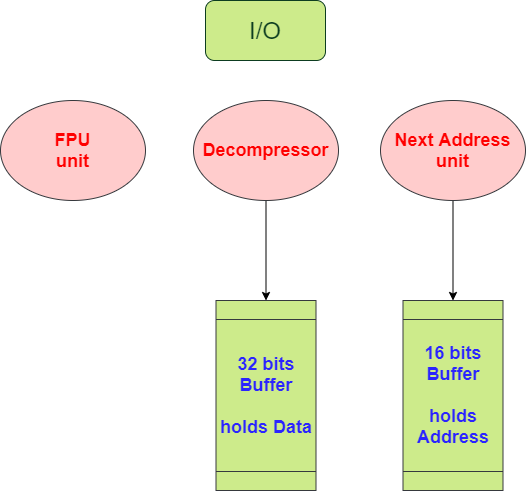
\includegraphics[width=\textwidth]{IO}
    \caption{I/O Internal Design}
    \label{fig:io}
\end{figure}

\subsubsection{Role}
\begin{itemize}
    \item Receive backets of 32 bits from the CPUm through \emph{DATA} bus.
    \item Decompress the data.
    \item Send the data to other modules (Solver/Interpolation/RAM).
\end{itemize}

\subsubsection{Ports}
\begin{itemize}
    \item INOUT: 32bit data bus with other modules.
    \item INOUT: 32bit data bus with CPU.
    \item IN: 16bit address bus.
    \item IN: CLOCK.
    \item IN: Reset.
    \item IN: 2bit Load/Process/Out.
    \item OUT: Interrupt to CPU.
    \item OUT: R/W to RAM.
    \item OUT: Error to CPU.
\end{itemize}

\subsubsection{Sub-modules}

\begin{itemize}
    \item {Decompressor}: see Section \ref{sec:decomp}.
    \item {Next Address Unit}: is responsible for calculating the next address to push the data at, as you know the address bus is our describer to the data on the data bus, so in order to let the IO knows where the matrix of variable ended this unit decides this, furthermore, {NAU} knows {N} and {M}, so when reading the matrix {A} it knows where exactly it ends.
    \item {FPU}: see Section \ref{sec:fpu}.
\end{itemize}

\subsection{Solver}

\begin{figure}[hp]
    \centering
    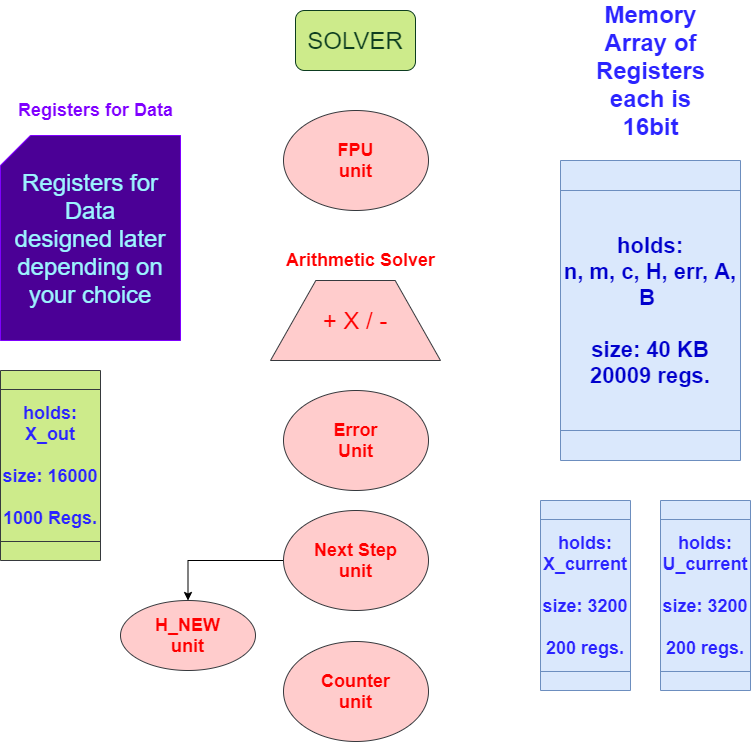
\includegraphics[width=\textwidth]{solver}
    \caption{Solver Internal Design}
    \label{fig:solver}
\end{figure}


\subsubsection{Role}
Receives $U_h$ from interpolator, gives it another $h$ to compute $U_{h_{new}}$ at, then computes $X_h$ and decides to stop and flush output to I/O or continue.

At the beginning it receives its data from I/O such as $N$, $M$, $err$, $h$ \dots etc.

\begin{itemize}
    \item Computes the upcoming X knowing h, the previous X and U.
    \item Counts the error difference and the new h.
    \item Checks for arithmetic errors that may occurs (e.g. div. by zero).
    \item Outputs the final X's at the desired times to the RAM.
\end{itemize}

\subsubsection{Ports}
\begin{itemize}
    \item IN: Done signal from interpolator.
    \item INOUT: 32bit data bus with other modules.
    \item IN: 16bit address bus.
    \item IN: CLOCK.
    \item IN: Reset.
    \item IN: 2bit Load/Process/Out.
    \item OUT: Interrupt to CPU.
    \item OUT: R/W to RAM.
    \item OUT: Error to CPU.
\end{itemize}

\subsubsection{Solver Memory}
\begin{itemize}
    \item Main Part: 40 KB $\rightarrow$ 20009 (16 bits) Registers
    \begin{itemize}
        \item N, M, C = 16 bits
        \item h = 64 bits
        \item err = 64 bits
        \item A = [50*50]*64 = 160000 bits
        \item B = [50*50]*64 = 160000 bits
    \end{itemize}
    \item $X_curren$t: 3200 bits $\rightarrow$ 200 (16 bits) Registers
    \begin{itemize}
        \item X = 50*64 = 3200 bits
        \item 50: max of M
        \item 64: max of numbers
    \end{itemize}
    \item $U_curren$t: 3200 bits $\rightarrow$ 200 (16 bits) Registers
    \begin{itemize}
        \item U = 50*64 = 3200 bits
        \item 50: max of M
        \item 64: max of numbers
    \end{itemize}
    \item $X_ou$t: 16000 bits $\rightarrow$ 1000 (16 bits) Registers
    \begin{itemize}
        \item X = 5 * 50 * 64 = 16000 bits
        \item 50: max of M
        \item 64: max of numbers
        \item 5: max of times answer is required
    \end{itemize}
\end{itemize}

\textbf{Note: main module stores all the 5 output values and flushes them to the CPU all at once at the end.}

\subsubsection{Sub-modules}
\begin{itemize}
    \item {FPU}: see Section \ref{sec:fpu}.
    \item {Error Unit}: to detect any error in sizes, h, numbers \dots etc.
    \item {Next Step Unit}: helps create the upcoming $h_{new}$ so that when solver is busy calculating $X_h$, interpolator is calculating $U_{h_{new}}$ \footnote{See Section \ref{sec:parallel} to learn more about parallelism.}, this unit represents the stepper unit, holds the logic of calculating the adaptive $h$, and detects when to stop, in summation it calculates the next $h$, even if it was fixed step.
    \item {Counter Unit}: tells you when to calculate more, when to advance to next time (in $T_s$), and when to stop the whole operations.
\end{itemize}

\subsection{Interpolator}

\begin{figure}[hp]
    \centering
    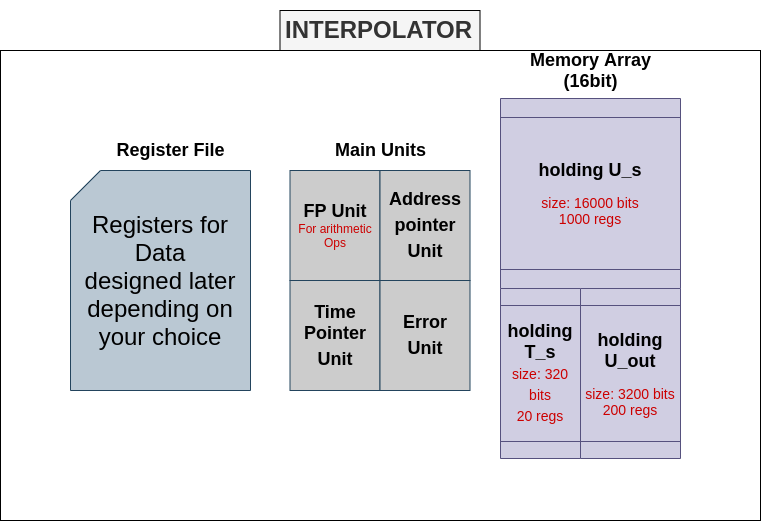
\includegraphics[width=\textwidth]{interpolator}
    \caption{Interpolator Internal Design}
    \label{fig:interpolator}
\end{figure}

\subsubsection{Interpolator Job Description}
\begin{itemize}
    \item Only computes U at a specific time.
    \item At the beginning it receives from IO the $U_s$ and $T_s$ fixed variables/data, and stores them.
    \item Each $U_s$ is at most of size [64*50] = 3200 bits = 200 registers
    \item Each $T_s$ is at most of size [64] bits = 4 regs.
    \item $T_s$ keeps hold of the time where each $U_s$ represents, for example, $T_s$ = [1, 2, 3], there fore the first 200 regs. In $U_s$ are the value of U at time 1, and so on... 
    \item You will need an iterator to target the appropriate $U_s$ from the array of memory, that's the \textbf{Address pointer Unit}.
    \item {Time Pointer Unit}: Identifies which $T$ of the $T_s$ array the unit is currently handling.
    \item Note: at the beginning of the program $T_{init} = 0$, $T_{final} = T_s[0]$, after a successful output, $T_{init} = T_{final}$, and $T_{final} = T_s[1]$, and so on...
\end{itemize}

\subsubsection{Role}
\begin{itemize}
    \item Calculates the upcoming U knowing h, U initial and U final.
\end{itemize}

\subsubsection{Ports}
\begin{itemize}
    \item OUT: Done signal to Solver.
    \item INOUT: 32bit data bus with other modules.
    \item IN: 16bit address bus.
    \item IN: CLOCK.
    \item IN: Reset.
    \item IN: 2bit Load/Process/Out.
    \item OUT: Interrupt to CPU.
    \item OUT: Error to CPU.
\end{itemize}

\subsubsection{Interpolator Memory}
\begin{itemize}
    \item $U_s$: 16000 bits $\rightarrow$ 1000 (16 bits) Registers
    \begin{itemize}
        \item $U_s$ = 5*[50]*64 = 16000 bits
        \item 50: max of M
        \item 64: max of numbers
        \item 5: max of times answer is required
    \end{itemize}
    \item $T_s$: 320 bits $\rightarrow$ 20 (16 bits) Registers
    \begin{itemize}
        \item $T_s$ = 5*64 = 320 bits
        \item 5: max of times answer is required
        \item 64: max of numbers
    \end{itemize}
    \item $U_{out}$: 3200 bits $\rightarrow$ 200 (16 bits) Registers
    \begin{itemize}
        \item U = 50*64 = 3200 bits
        \item 50: max of M
        \item 64: max of numbers
    \end{itemize}
\end{itemize}

\subsubsection{Sub-modules}
\begin{itemize}
    \item {Error Unit}: responsible for detecting when an arithmetic error may occur, like dividing by zero, \textbf{h} is getting bigger every time, different sizes....etc.
    \item {FPU}: see Section \ref{sec:fpu}.
\end{itemize}

\subsection{Fixed/Floating Point Unit (FPU)}
\label{sec:fpu}

\begin{center}
    \begin{figure}[hp]
        \centering
        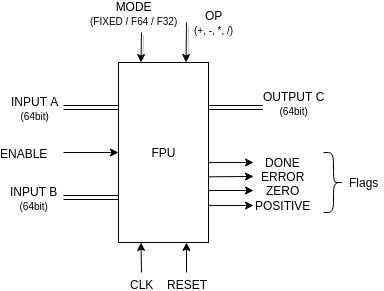
\includegraphics[width=\textwidth]{FPU}
        \caption{FP Unit}
        \label{fig:fpu}
    \end{figure}
\end{center}

\subsubsection{Role}
\begin{itemize}
    \item Instantiated, in the rest modules, multiple times and for different purposes.
    \item perform the following operations given in port \emph{OP}.
    \item perform them in different modes given in \emph{MODE}.
\end{itemize}
\subsubsection{Ports}
\begin{itemize}
    \item MODE: IN
    \begin{itemize}
        \item FIXED(0): operate on LOWEST 16bits of both A and B following Fixed point specifications.
        \item F64(1): operate on ALL 64bits of both A and B following Floating point specifications.
        \item F32(2): operate on LOWEST 32bits of both A and B following Floating point specifications.
    \end{itemize}
    \item OP: IN
    \begin{itemize}
        \item 0: $C = A + B$ 
        \item 1: $C = A - B$ 
        \item 2: $C = A * B$ 
        \item 3: $C = \frac{A}{B}$  
    \end{itemize}
    \item CLK: IN\\
        FPU operates on POSITIVE edge.
    \item DONE: OUT\\ 
    one operation needs multiple clocks, so FPU must RAISE DONE to 1 when finished for EXACTLY ONE clock cycle.
    \item ENABLE: IN\\
    FPU must only operate when ENABLE is set to 1.
    \item A, B: IN\\
    Input busses, all are 64bit wide.
    \item C: OUT\\
    Output bus, 64bit widw.
    \item ERROR: OUT
    \begin{itemize}
        \item FPU sets ERROR to 1 when an exception takes place. 
        \item Each mode has its possible set of exceptions, see the corresponding specifications. 
        \item MUST stay at 1 after setting it, until RESET is set to 1.
    \end{itemize}
    \item RESET: IN\\
    clears ERROR state REGARDLESS of ENABLE input.
    \item ZERO: OUT\\
    Set when output $C$ is zero.
    \item POSITIVE: OUT\\
    Set when output $C$ is positive, otherwise cleared.
\end{itemize}
\subsubsection{Fixed point specifications}
\begin{itemize}
    \item 16bit input
    \item 16bit output
    \item CONSTANT scale factor for both input and output = 7. see Subsubsection \ref{sec:fpu:scale}.
    \item in case of overflow or division by zero, ERROR MUST be set to 1 and MUST stay at 1 until RESET is set to 1.
\end{itemize}

\subsubsection{Floating point specifications}
\begin{itemize}
    \item MUST adhere to IEEE-754 2019-revision \cite{ieee754} for both fp32 and fp64 modes.
    \item ERROR is set to 1 when ANY of the exceptions stated in the IEEE-754 takes place, and stay at 1 until RESET is set to 1.
\end{itemize}

\subsubsection{Scale Factor Definition}
\label{sec:fpu:scale}
Scale Factor is an integer used to obtain the real number from the fixed point number and vice versa using the following formula: 
$y = \frac{x}{2^s}$; where: 
\begin{itemize}
    \item $x \in \mathbb{N}$ is the fixed point number stored as an integer.
    \item $y \in \mathbb{R}$ is the real number that represents $x$ with some error.
    \item $s \in \mathbb{N}$ is the scale factor.
\end{itemize}

\section{Compression}
Follow bit-level Run-length encoding to compress ram content before sending them, by taking each (one to eight) [1:8] repeating bits and compressing them into four bits, using RLE (Run length encoding) algorithm.

\subsection{Input}
Bit stream input data to IO.

\subsection{Output}
Y compressed 4bit packets, where $X \geq Y \geq \ceil{\frac{X}{8}}$
Each packet must follow the format in Table \ref{tab:comp-out}.

\begin{center}
    \captionof{table}{Compression Output\label{tab:comp-out}}
 \begin{tabular}{||c |l |c||} 
 \hline
 Bit Index & Description & Size \\ [0.5ex] 
 \hline\hline
  3:1 & Number of bits to generate - 1 & 3 bits  \\ 
 \hline
 0  & Bit to generate &  1 bit \\ [1ex] 
 \hline
\end{tabular}
\end{center}

\textbf{Note: the 3 bits must be incremented before decode.}

\subsection{Example}

\begin{center}
    \captionof{table}{Compression Example\label{tab:comp-exmp}}
 \begin{tabular}{||c |c||} 
 \hline
 Original & Compressed \\ [0.5ex] 
 \hline\hline
  11111111 & 1111 \\ 
 \hline
 0000  & 0110 \\ [1ex] 
 \hline
\end{tabular}
\end{center}

\subsection{Algorithm}
\begin{verbatim}
c = first bit in bit_stream
count = 0
for b in bit_stream:
    if c == b and count < 7:
        count++
    else:
        emit_packet(count-1, c)
        count = 1
        c = b
\end{verbatim}

\subsubsection{Compression Design Justification}
Because the occurence of more that 7 ones or zeros simultaneously is very rare.

\subsubsection{Problems}
This compression algorithm may not compress the data, rather than that it may increase the number of bits.

\section{Decompression}
\label{sec:decomp}
Follow this simple algorithm to fill the buffer, once its full (has 32bits) flush it to data bus and update the address.

\begin{verbatim}
for packet in packets:
    # bit to repeat
    b = packet[0]

    # extract 3 bits
    n = packet[3:1]

    # increment by 1 to get number of repetitions
    n++

    # generate n bit of b
    for _ in range(n):
        buffer.push(b)

    if buffer.full():
        buffer.flush()
\end{verbatim}

\part{Bibliography}
\begin{thebibliography}{9}
    \bibitem{mainDoc}
    \textit{ODE Solver -- System Description}. CMP Engineering Department, Cairo University. Spring 2020.
    \\\textit{\url{https://docs.google.com/document/d/1eHHQ9NC2HlrqLECSz6iQl5c6tR_y5AxtJBdxklAY5g4}}

    \bibitem{ieee754}
    Wikipedia contributors. (2020, March 15). IEEE 754. In Wikipedia, The Free Encyclopedia. Retrieved 19:00, March 21, 2020, from \\\textit{\url{https://en.wikipedia.org/w/index.php?title=IEEE_754&oldid=945680688}}
\end{thebibliography}

\end{document}
